\documentclass{article}
\usepackage[utf8]{inputenc}
\usepackage{amsmath}
\usepackage{amsfonts}

\usepackage{graphicx}
\usepackage{subcaption}

\usepackage{tikz}
\usetikzlibrary{shapes.geometric, arrows}
\usetikzlibrary{calc}
\usepackage{color}

\usepackage[backend=biber]{biblatex}
\addbibresource{pos_rk_stephan.bib}

\title{Positivity-preserving adaptive Runge-Kutta methods: results}
\author{Stephan Nuesslein}

\begin{document}

\maketitle


A big number of problems that preserve positifity reaction discretiesed PDEs...

With increasing complexity of the right hand side a step requect has a high cost. 
The goal of the project is to develop a positivity preserving method that uses adaptive b-Coefficients for every step.  This means that the computed stage values can be used and don't have to be recomputed. 
The resulting b should comply with the order conditions as far as possible.



(Note: The problem is connected to the theory about embedded methods, in the sense that one have different RKM with the same set of stage values. It may be interesting to have some literature regarding this)

Other Approaches: 
ssp104 methods: The idea is to construct a rkm Method out of explicit euler steps, that lead to a positive result for small enough $\Delta t$. (Todo: Read some literature regarding this and give a short explaination)

Implicit methods: Modified Patanka-Runge-Kutta (MPRK) \cite{kopecz_comparison_2019}

The idea of adapting the $b$ after calculation the stage values is used in \cite{ketcheson_spatially_2013}
In this case it is used to adapt the properties of the time integrator for a method of lines simulation on a PDE. With this approach it is possible to have different properties of the RKM at different parts of the domain. 


\section{Main Idea}

When computing the solution of an ODE $u ' = f(t,u) $ using a RK-Method with $s$ Stages the stage values $k^{(1)},\cdots,k^{(s)}$ are computed according to

\begin{equation}
k^{(j)} =  f(t^n + \Delta t c_j, u^n + \Delta t \sum_{l = 1}^{s} a_{jl} k^{(l)}  \quad j = 1,\cdots,s)
\end{equation}

Based on these values the next solution $u^{n+1}$ is computed by

\begin{equation}
u^{n+1} = u^n + \Delta t \sum_{j  = 1}^s k^{(j)} b_j .
\end{equation}

This equation can be formulated to

\begin{equation}\label{eq:Combination}
u^{n+1} = u^n + \Delta t K b
\end{equation}

where $K$ is a matrix containing the stage values $k_1,\cdots,k_s$.

One reason why steps are requected is that the new solution $u^{n+1}$ does not comply with positifity. 
So it may be adventagious to adapt Equation\,\ref{eq:Combination} in such a way that $u^{n+1}$ is positive. This is done by adapting the weights $b$.
As it can be see in Equation\,\ref{eq:Combination} $u^{n+1}$ is a linear combination of the stage values and the previous solution $u^n$.
When altering the weights the properties of the RKM should be preserved. Especially the Order of the RKM.  
To ensure this the Order Conditions should be still meet. 
Because the coeffeicents $a_{jl}$ are already fixed the Order Conditions reduce to linear equations.
This means that finding the $b$ can be done by solving a linear Programming problem.
 
This approach to ensure positifity preserves linear invariants like mass conservation, because it is a regular RKM. 
If there are no negative values in $u^{n+1}$ with the original $b$, then the method does not cause additional effort, because it only has to solve the LP-Problem if the regular RKM does not lead to a positive $u^{n+1}$. (exept for the test)
No additional evaluations of the rhs.

Flowchart to evaluate a step:

\begin{itemize}
\item Calculate the stage values $k_1,\cdots,k_s$
\item Calculate the $u_{n+1} = u_n + \Delta t K b_{d}$ with a default b
\item Test $u_{n+1} \geq 0$, if not:
\item find a new b with $u_n + \Delta t K b \geq 0$
\item Calculate the $u_{n+1} = u_n + \Delta t K b$ with the new b
\end{itemize}


\section{Applicable Problems}
The approach can be used with ODE systems $u' = f(t,u)$ that ensure  $u(t) \geq 0 \forall_t \forall_{  u_0 \geq 0}$ 

This can be tested with the property 
\begin{equation}
u_i=0 \Rightarrow f_i(t,u_1,\cdots,u_i,\cdots,u_n) \geq 0  \forall_{u_c \geq 0} \forall_{t}
\end{equation}

For problems where only the combination of $f(t,u)$ and $u_0$ leads to the positifity of the exact solution, tests did not show promising results. Additional it is not certain if the computed solutions would be reasonable.

\section{Details}

\subsection{Positifity}

For the further discussion we are concerned with a System of $m$ coupled ODEs. 
In this setup  $u \in \mathbb{R}^m$.
Systems of ODEs with a high number of dimensions can appear when solving a PDE with the method of lines.

To enshure that the solution is positive 

\begin{align}
 u_i^{n+1} &\geq 0   \;   \forall_{i \in \{1, \cdots,m \}}  \\
 u_i^n + h \sum_{j=0}^{s-1} b_j h_i^j  &\geq 0   \;   \forall_{i \in \{1,\cdots,m \}}  
\end{align}

has to be fulfilled.
This infers $m$ positivity constraints to the optimisation problem. These can be written as

\begin{equation}
u_i + \Delta t K  b \geq 0     
\end{equation}

where $K = \big[k^1 , \cdots k^{s-1}\big]$.

This causes unnecessary many inequality constraints on the LP-Problem. To simplify the problem one want to reduce the number of positifity constraints by ignoring it for ODEs where there is no issue with positifity.

The new positifity constraints can be formulated as
\begin{equation}
u_i^n + \Delta b \sum_{j=0}^{s-1} b_j h_i^j  \geq 0   \;   \forall_{i \in h \subseteq \{1,\cdot,m \}} 
\end{equation}

For this a set $h \subseteq \{1,\cdots,m \}$ that include all indecies that are needed for determining the $b$ has to be chosen.

A reasonable approach is to set $h_0 = \{ i \in \{1,\cdots,m \} |  u_i^{n+1}  < 0 \}$. 
After the new $b$ and $u^{n+1}$ is computed using $h_0$, the algorithm has to check if the positifity of the other values $i \notin h_0 \subseteq \{1,\cdots,m \}$ is still meet. 
If the conditions is not meet a new set $h_{a+1} = \{ i \in \{1,\cdots,m \}|  u_i^{n+1}  < 0 \} \cup h_{a}$ using the new $u^{n+1}$ is generated and the LP-Problem is solved again. This process id repeated until a solution is found that leads to a $u^{n+1} \geq 0$. The choice of $h_{a+1}$ based on the $h_{a}$ ensures that the algorithm cannot get stuck in a loop. In the worst case $h_a$ is growing very slowly until $h_a = \{1,\cdots,m \}$. 

This effect did not occur so far. A approach on this would be to make a educated guess which indecies could get a problem with positifity. A possible estimate would be $\frac{u_i^{n+1}}{max(K_{(i,0)}, \cdots ,K_{(i,0)})} $ 

When enforcing a maximum value the number of constraints can be reduced using the same technique. When both enforcing maximum and minimum values two separate sets of active constraints $k_{min}$ and $k_{max}$ are used. The set $k_{max}$ denotes the active maximum constraints and the set $k_{min}$ denotes the active minimum constraints. 
Here it is important to update these sets simultaneously.  


\subsection{Order Conditions}\label{sec:OrderCond}

The Order Conditions for a RKM are a set of Equations depending on $a_{jl}$, $c_1,\cdots,c_s$ and $b_1,\cdots,b_s$. In these Equations $b_1,\cdots,b_s$ only appear linearly \cite{hairer_runge-kutta_1993}.
If $a_{jl}$ and $c_1,\cdots,c_s$ are already known, the Order Conditions for the Order $p$ are an linear equations system and can be written as $Q b = r$. 

The vector $b \in \mathbb{R}^s$ contains the weights and $Q$ is an $n \times s$ matrix, where $g$ is the number of Order Conditions. The vector $r$ contains the right hand side of the Order Conditions.

If the $A$ of a  preexisting RK-method is used, there is at least one solution for the linear equation system.
In order to get an optimization problem the equation system has to be underdetermined.
This implies that $\mathrm{rank}(Q) < s$. 
Because the Quadrature Conditions are linear independent, there are at least $p$ independent vectors in $Q$. This leads to the condition $p < s$.
This implies that the number of stages has to be higher as the wanted order.


\subsection{Ways to formulate the Optimization Problem}

There are two possible ways to write down the adaptation of the $b$. The first way is to directly adapt the original weights $b_{orig}$ by adding a correction $\Delta b$ that ensures positivity.
This is the easiest way to adapt the $b$. An advantageous property is that the step size can be reduced after calculation the stage values by using the dense output order conditions.  
(Note: Recommendation for explicit methods)
The direct adaption approach is explained in more detail in section\,\ref{sec:direct}.

The second approach is to choose $b$ as a convex combination of a set of $b$s. This approach is more useful if some embedded methods with certain properties are know. 
This approach also shows more  predictable behavior because the resulting $u^{n+1}_b$ is also a convex combination of the solutions $u^{n+1}_{b_a},u^{n+1}_{b_b},\cdots$ 
(Note: Recommendation for implicit methods)
The direct adaption approach is explained in more detail in section\,\ref{sec:convex}

Both approaches are shown in figure\,\ref{fig:b_space}.


\begin{figure}
    \centering
    \begin{subfigure}[b]{0.45\textwidth}
        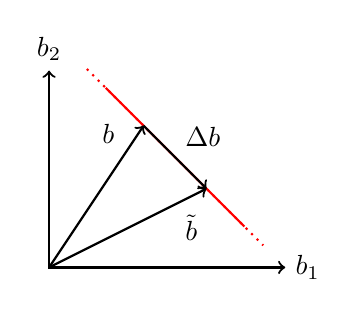
\begin{tikzpicture}
    % Draw axes
	\coordinate (borig) at (1.2,1.8);
    \coordinate (b) at (2,1);
	\coordinate (db) at ($(b)-(borig)$);

    \draw [<->,thick] (0,2.5) node (yaxis) [above] {$b_2$}
        |- (3,0) node (xaxis) [right] {$b_1$};


%Add subspace 
	\draw[thick,red,dotted] ($-0.9*(db)+(borig)$) -- ($0.9*(db)+(b)$);
	\draw[thick,red] ($-0.6*(db)+(borig)$) -- ($0.6*(db)+(b)$);
	
	\draw[thick,->] (borig) -- node[anchor=south west ,pos = 0.5] {$\Delta b$} (b);
	\draw[thick,->] (0,0) -- node[anchor=south east,pos = 0.8] {$b$} (borig);
    \draw[thick,->] (0,0) -- node[anchor=north west,pos = 0.8] {$\tilde{b}$} (b);

\end{tikzpicture}
        \caption{Direct Adaptation}
        \label{fig:b_direct}
    \end{subfigure}
    \begin{subfigure}[b]{0.45\textwidth}
        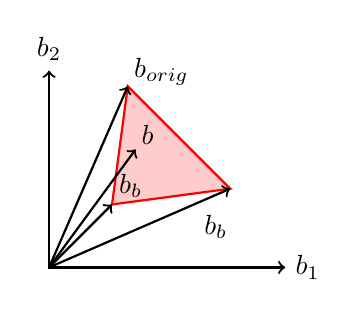
\begin{tikzpicture}
    % Draw axes
	\coordinate (borig) at (1,2.3);
    \coordinate (b_a) at (0.8,0.8);
	\coordinate (b_b) at (2.3,1);
	\coordinate (b) at (1.1,1.5);


    \draw [<->,thick] (0,2.5) node (yaxis) [above] {$b_2$}
        |- (3,0) node (xaxis) [right] {$b_1$};

    \draw[thick,red,fill = red!20] (borig) -- (b_a) -- (b_b) -- cycle;

	\draw[thick,->] (0,0) -- node[anchor=south west,pos = 0.95] {$b_{orig}$} (borig);
    \draw[thick,->] (0,0) -- node[anchor=south west,pos = 0.95] {$b_b$} (b_a);
    \draw[thick,->] (0,0) -- node[anchor=south west,pos = 0.95] {$b$} (b);
	\draw[thick,->] (0,0) -- node[anchor=north west,pos = 0.8,fill=white] {$b_b$} (b_b);

\end{tikzpicture}
        \caption{Convex Combiantion}
        \label{fig:b_convex}
    \end{subfigure}
    \caption{Graphical representation of the two different approaches to adapt the weights}\label{fig:b_space}
\end{figure}

\subsection{Direct Adaptation}\label{sec:direct}

When directly adapting the $b$ a new $b$ that complies with the Order Conditions is chosen.   
The weights $b = b_{orig} + \Delta b$ consist of the weights of the original method $b_{orig}$ and an adaption $\Delta b$. This $\Delta b \in \mathrm{ker}(Q)$. 
In Figure\,\ref{fig:b_direct} this is is drawn. The red line represents the subspace of $b$ that compile with the Order Conditions. Both $b_{orig}$ and $b$ are in this subspace. 
 
To run it as a LP-Problem a set of constraints is constructed.  
Also a objective function is needed to determine the optimal $b$.

\subsubsection{Constraints}
The Direct Adaptation approach leads to two set of constraints on the $b$.

The first set of constraints is the positifity and can be written as 
$$u_{n+1}=u_n+\Delta K \vec{b} \geq 0$$

The second set of constraints are the Order Conditions
$$Qb=r$$



\subsubsection{Objective Function}
Different types of objective functions have been tried. 

\begin{description}

\item[L1 norm] The optimisation Problem opimises for $min(|b-rkm.b|_1)$
            
\item[Quadrature]   The optimisation Problem opimises for $min(|b^Tq-r|)$
                            where q is the quadrature condition of the next higher order 
                            and r is the expected right hand side
            
\item[Hom. Order]    The optimisation Problem opimises for $min(|bTO|)$ where O are the homogenus Order Conditions of the next higher orders
                            
 
\end{description}

A reasonable property of the objective function would be that for the LP-Problem only constrained by the order condition the optimal solution is $b = b_{orig}$. 
This can be achieved by $argmin(f_{optim}(b)) = b_{orig}$. 
In practice this also means that there is no need to solve solve the optimization Problem if no constraints are violated because the solution of this problem is already known. This is adventagious for performance reasons.
The different approaches have been tested on a linear test problem from \cite{kopecz_unconditionally_2018}. The optimization problem was used at every step.
The magnitude of $b$ can get large if the Order Conditions are used as objective function.
Large values of b can lead to numerical instability. Because $\sum_{i  = 1}^s b_i = 1$, a increase of $||b||$ leads to a combination of negative and positive values. Because the computation only is done with a finite precision (and usually in floating point) large $||b||$ can lead to absorption effects.    
By changing the $b$ the stability function is altered. This can lead to oscillations if the poles of the RHS are no longer in the stability region of the resulting method.
For these reasons $||b-b_{orig}||$ seems like a good choice. The 1-Norm can be implement the with Linear Programming using slack variables. We choose $||b_{optim}-b_{orig}||_1$ as objective function.




\subsubsection{Adaption of Timestep using the dense output formual}

If the original step $\Delta t$ was to large and there is no suitable $b$, we would like to calculate a $u^{n+1}$ using the stage values instead of rejecting the step. For this the time step is reduced after calculation the stage values. This can be done using the Order Conditions for dense Output. These can be found in \cite{hairer_runge-kutta_1993}.
We introduce $\theta \in (0,1]$. The new step taken has the length $\theta \Delta t$ whereas $\Delta t$ is the time step used when calculating the Stagevalues.
To calculate a reduced step the Order Conditions have to be adapted and a new $b_{orig}$ for the objective function (and more important the Error detection afterwards) has to be generated. 
(TODO: the $b_{orig}$ is still a open question)

When adapting the Order Condition to a new $\theta$ the Order Condition Matrix $Q$ stays unchanged whereas the right hand side depends on $\theta$.

The dependency of $r(\theta)$ is nonlinear. This means that the maximum $\theta$ with a suitable $b$ can not be calculated by solving a LP-Problem. This means that different $\theta$ have to be tested independently. 
(Note: we could include some algorithm to search for it)


\subsection{Convex combination of existing methods}\label{sec:convex}
For some test problems (e.g. the Heat Equation solved with an implicit method), large distortions occur, even though a norm of the distortion of the b is used as a objective function. 
For implicit methods it is known that implicit euler steps lead to a positive solution for any $\Delta t$. The backward Euler is still only first Order but shows more exact results in certain cases than a method of higher Order that shows distortions of the solution caused by the larger error coefficients ($\Delta t \gg 0$, so they do not disappear because of the nature of the polynomial).
A possible method to fix this is to generate the new b based on a convex combination of embedded methods of RKM. 

\subsubsection{Constraints}
At first a set of embedded methods of the RKM $b_1,\cdots,b_d$ are needed. 
If all the used b complies with an order conditions the new method also has this order.
This can is straightforward using

$$ q^T b = q^T (\chi b_{\alpha} + (1-\chi) b_{\beta}) = \chi q^T  b_{\alpha} + (1-\chi) q^T  b_{\beta}) = \chi rhs + (1-\chi) rhs = rhs$$

The new $b$ is defined as 
\begin{equation}\label{eq:b_convex_def}
\vec{b} = \sum_i^d a_i \vec{b_i} = Ba
\end{equation}


where $B=\left[b_1,\cdots,b_d \right]$ is a matrix containing the embedded methods.  
To ensure the that Equation\,\ref{eq:b_convex_def} yields a convex combination following constraints are enforced for the  the parameters $a,\cdots,a_d$.

\begin{equation}
 0 \leq a_1 \leq 1  \forall_{i \in \{1, \cdots d \}}
\end{equation}
\begin{equation}
 \sum_{i=1}^d a = 1
\end{equation}


The positifity constraint changes to 

$$u_{n+1}=u_n+\Delta K B a \geq 0$$


\subsubsection{Objective Function}

As an Objective function the function

$$ min \left(\sum_i^d w_i a_i \right) $$

is used.  The $w_1,\cdots,w_d$ are weighting factors that determine which is the preferred $b_i$ to use.

Because the optimal solution of the unconstrained problem has to be the original $b$ the weight $w_0$ corresponding to $b_{orig}$ should be the smallest $w$. This weight is simply set to $w_{b_{orig}} = 0$. For the other weights $w_i = \frac{1}{\mathrm{Order} \{b_i\}}$ is used.

\subsubsection{Construction of Embedded Methods}
For methods with $s \geq p$ it is useful to have some degrees of freedom for the highest order. For this at least one $b$ that complies with the order Condition of the highest order and $b \neq b_{orig}$ has been introduced.
These additional $b$ can be constructed by calculating a Span $S$ of the Kernel $\mathrm{ker} (Q)$ of the Order Condition Matrix $Q$. For every vector $s \in S$ one set of weights with $b = b_{orig} + a s$ and one with $b = b_{orig} - a s$ is added. The $a$ is a parameter that determines how big a change is allowed. 

As a first order method a $b$ is added that corresponds to a series of backward euler steps. These are know to be yield to a positive result (Todo: source).

An important property of the embedded methods is that they should show the desired stability characteristics.

A Reduction of the step size suing the order Conditions for dense output would also be possible. For this a set of embedded methods $b_1(\Theta),\cdots,b_d(\Theta)$ has to be constructed. This was not done in this research.

(Note: Doing dense Output here is a bit complicated, but it would not help ensure positifity only (maybe) increase exactness.  is it worth exploring this or is it better to just leave this open for further research it may be also interesting regardless the study of positifity)
Everything has downsides...
 


\subsection{Choice of Baseline Method}
An important property for the used baseline method is the Existence of embedded methods and the degrees of freedom for the b.
As noted in Section\,\ref{sec:OrderCond} the number of Stages has to be higher than the Order. 
Another important property is the number of degrees of freedom for the choice of the new weights. 
These can be calculated using $s-\mathrm{rank}(Q)$%$\mathrm{dim}(\mathrm{ker}(Q))$.
The number of degrees of freedom for different methods are shown in table\,\ref{table:DOF_exp} for explicit methods and in table\,\ref{table:DOF_imp} for implic methods.

\begin{table}[h!]
\centering    %Generated below============ 
\begin{tabular}{|l |c c c c c c |} 
 \hline 
Order &1&2&3&4&5&6 \\ 
 \hline Classical RK4&3&2&0&0& - & -  \\ 
 SSPRK(10,4)&9&8&6&4& - & -  \\ 
 Cash-Karp RK5(4)6&5&4&2&1&0& -  \\ 
 Dormand-Prince RK5(4)7&6&5&3&1&0& -  \\ 
 \hline 
 \end{tabular}
 \caption{Degrees of Freedom for Choice of $b$} %Generated above============ 
 \label{table:DOF_exp}
 \end{table}
 
 \begin{table}[h!]
\centering   %Generated below============ 
 \begin{tabular}{|l |c c c c c c |} 
 \hline 
Order &1&2&3&4&5&6 \\ 
 \hline Implicit Euler&0& - & - & - & - & -  \\ 
 Im-Euler 2&2&1& - & - & - & -  \\ 
 Im-Euler 3&5&4&2& - & - & -  \\ 
 Im-Euler 4&9&8&6&3& - & -  \\ 
 \hline 
 \end{tabular}
 \caption{Degrees of Freedom for Choice of $b$} %Generated above============ 
 \label{table:DOF_imp}
 \end{table}


For all methods with the number of stages equal to the order of the method, there are no degrees of freedom without reducing the order. 
If the Classical RK4 method is used the Order has to reduced more because the RK4 method does not have embedded methods of order 3.
Contrary to this methods with $s > p$ have degrees of freedom even without reducing the order. 

Another important property is the stability region in comparison with the maximum $\Delta t$ that ensures positifity. For this approach to be useful the RK-method has to yield negative results for $\Delta t$ smaller than the biggest stable $?Delta t$.

(Note: up to this point i do not understand why this is happening. We only see it occur depending on the Proble-RKM combination)

A third property is the existence of a positive solution. This corresponds to the question if there is a embedded first order method that ensures positivity. This is particularly interesting for Implicit methods, because the $\Delta t$ is not limited by the stability. 
If we have a embedded first Order Method we can ensure that there is always a positive solution, which might be of first Order. (Todo: Source)

\subsection{Error detection/Approximation}
(Todo: edit this whole section, Add some mathematically more rigorous statement)

The main question is: We see that for certain $b$ that comply with the Order Conditions we get results that do not resemble the solution. (some type of glitches, artefacts)

Note: in general it is difficult to give some mathematically rigorous statement for this statement because -by definition- it only applies for $\delta t \gg 0$ where the proofs using the Taylor Series do not give valid results any more. We could say that the main idea of the adaption of $b$ is to alter the error in a certain way that we know that the numerical solution gets 'better' in the sense that it only leads to positive solutions. 
When taking the Taylor Series of the numeric solution the coefficients up to the Order of the method are fixed by the Order Conditions. The only degrees of freedom are the coefficents above the Order Conditions. This requires that $\Delta t > 0$. (More like $\Delta t^n \approx \Delta t^(n+1) $)
The main way is to ensure that for $\Delta t \to 0$ : $b \to b_{orig}$. For this case we already know that the numeric solution converges to the exact solution.  
This is made sure by property of the Objective function that $argmin(f_{optim}(b)) = b_{orig}$. 

To make sure that the new adapted solution is still reasonable we measure the deviation form the Original method. In the worst case the errors add up. (todo: here some math formula... (We know that can not be the case because we already know that we will reduce the error for the quantity we will make positive, still we can use it as a upper bound.))


\subsection{Stability Region}

By adapting the $b$ the used RK Method is changed. This also alters the stability function and therefore changes the region of absolute stability. 
It depends on the solved problem, the RKM and the used $\Delta t$ on how many steps the stability function is altered. For Problems where only a small number of step are affected a bigger change in the stability function would be acceptable. For Problems with require a adaptation of the weights for every step one needs to make sure that the resulting method is stable.


In \ref{proof:combiningb} it is stated that one can construct the stability function of a RKM  $R_b$  with the weights $b = \alpha b_1 + \beta b_2$ by adding the weighted stability functions $R_{\alpha b_a+\beta b_b}(z) = \alpha R_{\alpha b_a}(z) + \beta R_{\beta b_b}(z) $ where all stability functions have the same $A$ and $\alpha + \beta = 1$.

(Todo:It is not straightforward if there are no pole zero cancellations in the stability function. For explicit methods the stability function is a polynomial o degree $\leq s$ (Hundsdorfer). Pole zero cancellations can not happen for these. For implicit functions that are A-stable the poles have to be in the right halve plane. Here is starts to get interesting. Because the A-Stability of one method with a certain $A$ is not a sufficient  condition that there are no Poles for all RKM with this A-Matrix. But it is possible (or easy) to prove that if $a_{ii} > 0 \forall i = 1,\cdots , s$ then there are only poles in the right halve plane where they do not matter for the further considerations.)



\subsubsection{Convex Combination}
If the new $b$ is a chosen as a convex combination of $b$ it is easy to prove that the resulting  the Region of absolute stability is at least the Intersection of the region of absolute stability of the methods that define the convex combination. (Compare Section\,\ref{proof:convex_comb}). This also means that if all the used embedded methods used to construct the new $b$ are A-Stable, the resulting method is also A-Stable.


\subsection{Direct Adaptation}
If the $b$ is adapted directly there is no such proof.
A useful property of the resulting stability region is that it is similar to the stability region of the baseline method. 
(Note: is it possible to give some statement like: If the stability regions of the rkm used for multiple steps are similar, then the overall method is stable for the intersection of the stability regions)

In Section\,\ref{sec:deriv_sr_b} a proof is given that for most methods a small change of $b$ does not alter the stability function dramatically.






\section{Implementation aspects of the Algorithm}

(Todo: Maybe a flowchart and a description on how we stitch everything together.) 

The algorithm on adapting the b consists of two main loops. The outer loop loops through all the $\theta$, staring with $\theta = 1$ down to the lowest $\theta$. The inner loop loops through the orders, starting with the highest Order down to the lowest Order. 
Until a acceptable $b$ the algorithm tests combiantions of $\theta$ and $p$. At first the Order Conditions are constructed. On these a LP-Solver is invoiced. If the LP-Problem is infeasible the algorithm immediately tries the next combination. If the LP-Problem is feasible we test if the $b$ is acceptable. At first it is tested weather the new $u^{n+1}$ indeed complies with the constraints. This is necessary because sometimes the used LP-solvers incorrectly identify the problem as feasible. (Note: because of the chosen objective function it can not be unbounded) As second test the deviation from the old solution (Compare Error estimation) is calculated. If the error is bigger than a set maximum error the $b$ is also rejected and the algorithm also switch to the next combination.
As soon as the algorithm finds a suitable $b$ the loops are aborted and the $b$ is used for the update step.
If all the combinations of $\theta$ and $p$ did not lead to a acceptable $b$ the step has to be rejected and a new set of stage values has to bee computed.

(Note: It would also be possible to use another strategy for traversing all the combinations of $(p,\theta)$. Is it worth exploring these? Eg, a visect algorithm for $\Theta$ or linear approximations)

(Note: Is here a good place to give a note on where supplementary code can be found?)

(Note: Should we discuss which solver is used. Probably it is not worth using space for some plot etc. on this... Maybe a short note?)



\section{Results of experiments}
\subsection{Explicit methods}
For most of the test problems problems with stability occur before getting negative values. This means that we need methods with large stability region.

\subsubsection{ADP}
A test problem that works good is the advection‐diffusion‐production‐destruction systems. 
For the production‐destruction systems negative values at the intermediate steps occurred. These results of these could be suppressed by the optimization problem  except for some timesteps where these yield to glitches in the solution.

Conclusion: it is important to control for negative Values in the intermediate stages.
Possible solutions: Solve an positifity ensuring optimization Problem at every intermediate step.
Can be formulated as choosing a new $b$ for every intermediate stage which then gets part of $A$ in the next step.

Another idea to explore (Is kind of obvious but could also be stupid): Replace $f(t,u)$ with an $f_{pos}(t,u)$ with 
$f(t,u)=f_{pos}(t,u) \forall u \geq 0 $
Whereas $f_{pos}(t,u)$ is welldefined for $u \leq 0$


We are going to test the solvers for multiple $\Delta t$. For the explicit method we want to show the important times.

$$ \Delta t \; \underset{0}{+}---------\underset{\Delta t_{pos}}{+}\underbrace{--------}_{\gamma}\underset{\Delta t_{feasible}}{+}---\underset{\Delta t_{stable}}{+}--->  $$

\begin{itemize}
\item
$\Delta t_{pos}$ is the largest stepsize that yields to positive results without adapting the $b$

\item
$\Delta t_{feasible}$ is the largest stepsize that can be used with the adaptive $b$

\item
$\Delta t_{stable}$ is the largest stepsize for that the method is stable
\end{itemize}


The timesteps where the adaption of the b is usefull is denoted with $\gamma$ idealy this interval is as large as possible. This means that $\Delta t_{pos} \ll \Delta t_{feasible} \approx \Delta t_{stable}$

With stepsizes $\Delta t > \Delta t_{stable} $ we cann not expect the solution to be reasonable

$\Delta t$ for the ADP Problem 

\begin{tabular}{|c|c|c|c|c|}
\hline 
Method & $\Delta t_{pos}$ &$\Delta t_{stable}$& $\Delta t_{feasible}$  \\ 
\hline
fe & 0.0015 & --- &  0.0051 \\
\hline 
ssp104 fallback =1 & 0.0134 & 0.0309 & 0.0311 \\ 
\hline 
dp5 &0.0031 &0.0031 & 0.0031\\ 
\hline 
ck5 & 0.0044&  0.0044 & 0.0044\\ 
\hline 
merson4 fallback= 1& 0.0038& 0.0055 & 0.0084\\
\hline
\end{tabular} 

We can see that for the ssp104 method is a good choice for this approach when solving this testproblem.  The merson4 method is also suitable. We can not get benefits form dp5 and ck5.


\subsubsection{Quantum Simulations}
Shows following shortcomings:

To ensure positifity we do not only need $\rho_{i,i} \geq 0$ but also the additional constraint $|\rho_{j,k}|^2 \leq \rho_{j,j} \rho_{k,k}$ at least for the elements with $j = k +1$ and $j = k-1$. This conditions can not be formulated as LP-Problem.

\subsection{Implicit methods}
Implicit methods seem like an advantageous choice for a couple of reasons.

\begin{itemize}
\item The computational effort of solving the optimisation Problem is relatively small compared to the overall cost of the method.
\item Implicit methods are stable for large step sizes.
\item Implicit methods ensure positifity for the backward euler step, even for large step sizes.
\item There are no methods for ensuring positifity for higher order methods (Which we also can not get around for the general case)
\end{itemize}

Used for the ADP model the model yields good results, the main limit for the stepsize is the accuracy of the solver for the stageequations.

When tested on the diffusion equation with an spike as initial data the $b$ is only changed for the first step. The change of the $b$ can lead to reasonable changes of the hight of the maximum. 



\section{Useful proofs}

\subsection{Existence of b}
Ensuring a feasible $b$ exists for a certain order condition is in general very difficult.
If we drop the order conditions it is known that there is a positive solution as long as there is a $k_c$ with $k_c \geq 0$.
This is no problem when using a implicit method because a backward euler step always gives a positive solution. 

\subsection{Stability function of linear combinations}\label{proof:combiningb}
Let $R_b(z)$ denote the stability function of a RKM method with the butcher tableau

$$
\begin{array}
{c|c}
c & A\\
\hline
& b^T
\end{array}
$$

We want to prove that $R_{\alpha b_a+\beta b_b}(z)$ = $\alpha R_{ b_a}(z)+\beta R_{b_b}(z)$ when $\alpha + \beta = 1$ and $A$ is the same for all methods.

We start with the definition of the RKM

\begin{align}
u_{n+1} &= u_n + \Delta t K (\alpha b_a+\beta b_b) \label{eq:u_n+1}  \\
u_{n+1}^{sum} &= \alpha (u_n + \Delta t K b_a) + \beta (u_n + \Delta t K b_b) \label{eq:u_n+1_sum} \\
& = (\alpha + \beta) u_n + \Delta t \alpha K b_a + \Delta t \beta K b_b \\
&= u_n + \Delta t K (\alpha b_a+\beta b_b) \\
&=u_{n+1} 
\end{align}

Now we insert the Stability functions for \ref{eq:u_n+1} and \ref{eq:u_n+1_sum} which we already know to be equal. We get 

\begin{align}
u_{n+1} &= u_{n+1}^{sum} \\
R_{\alpha b_a+\beta b_b}(z) u_n &= \alpha R_{\alpha b_a}(z) u_n + \beta R_{\beta b_b}(z) u_n \\
&= (\alpha R_{\alpha b_a}(z) + \beta R_{\beta b_b}(z)) u_n
\end{align}

because this has to be true for all $u_n$ we get

\begin{equation}
R_{\alpha b_a+\beta b_b}(z) = \alpha R_{\alpha b_a}(z) + \beta R_{\beta b_b}(z) 
\end{equation}

\subsection{Stability of convex combination}\label{proof:convex_comb}

With this we can proof that the convex combination of two methods is absolutely stable at the points where both original methods were absolutely stable.

We want to show that $(|R_{b_a}(z)|  < 1) (|R_{b_b}(z)| < 1) \Rightarrow |R_{\chi b_a +(1- \chi) b_b}(z)| < 1$ with $\chi \in [0,1]$.
We write $\alpha = \chi$ and $\beta = 1-\chi$ for convenience.

\begin{align}
|R_{\alpha b_a +\beta b_b}(z)| &= |\alpha R_{b_a}(z) + \beta R_{b_a}(z)| \leq |\alpha R_{b_a}(z)| + |\beta R_{b_a}(z)|\\
 &=| \alpha| \underbrace{|R_{b_a}(z)|}_{<1} + |\beta| \underbrace{|R_{b_a}(z)|}_{<1} < \alpha + \beta = 1
\end{align}


\subsection{Stability of direct adaptation}\label{sec:deriv_sr_b}

We would like to calculate the derivative of the border in respect to a change of $b$. 



The stability function depending on the $b$ is expressed (Note: it is a bit complicated her because we cannot let it depend on the b directly, but only give b after a coordinate transformation, which also makes the expression easier because we can already introduce the order conditions here)
$m$ is the number of dimensions of the Kernel of the Order Condition $m = \mathrm{dim}\{\mathrm{Ker} (Q) \}$
The $b_1,\cdots,b_m$  are the Basis vectors of $\mathrm{Ker} (Q)$. By this we can get the vector $w$ by $w = \left[b_1,\cdots,b_m\right]^{-1}(b-b_{orig})$.

The General Stability function of all embedded RKM that satisfy the Order Conditions $Q$ is given by 

\begin{equation}\label{eq:gen_stabilityf}
R(w,z) = (1-(w_1,\cdots,w_m))R_{b_{orig}}(z) + w_1 R_{b_1}(z) + \cdots + w_m R_{b_m}(z)
\end{equation}

The border is defined by the implicit function 
\begin{equation}\label{eq:border}
|R(w,u+iv)|^2 -1 = 0
\end{equation}
This function can be viewed either as $\mathbb{R}^m \times  \mathbb{C} \rightarrow \mathbb{R}$ or $\mathbb{R}^m \times  \mathbb{R}^2 \rightarrow \mathbb{R}$.
We are only concerned with the expansion or contraction. Because of this we are only interested in the change perpendicular to the Border of the stability region. 

For a point $z_0= u_0 +i v_0 $ 
with $ |R(w,z_0)|^2 -1 = 0 $ the gradient of
 $|R(w,u,v)|^2$ is calculated. 
If the gradient does not vanish at $z = z_0$ Equation\,\ref{eq:border} Can be transformed in a function $\mathbb{R}^m \times \mathbb{R} \rightarrow \mathbb{R}$ depending on $w$ and a single variable $a$ by setting $z = z_0 + n a$. The complex number $n$ denotes the normal vector $\vec{n} = \frac{\nabla |R(w,u,v))|^2}{\left| \nabla |R(w,u,v))|^2 \right|}$ of the border of the stability region written in complex notation. This defines the function $a(w)$ with $|R(w,z_0 + n a(w))|^2 -1 = 0$. 
This implies that this approach is only applicable if the gradient does not vanish on the border of the stability function. This is not true in general but for the most common RKM.
The derivative $\frac{\mathrm d}{\mathrm d w} (a(w))$ can be calculated using the implicit function theorem. The defining function is 
\begin{equation}\label{eq:f(w,a)}
f: \mathbb{R}^m \times \mathbb{R} \rightarrow \mathbb{R} f(a) = |R(w,z_0 + n a)|^2 -1 
\end{equation}

If explicit methods are used this function is known to be continuously differentiable because it can be written as a Polynomial of $w_1,\cdots,w_m,u$ and $v$. This is a necessary condition for the use of the of the Implicit function theorem. 
It is also known by definition, that for the point $w=0$ and $z = z_0$ the equation $ |R(w,z_0)|^2 -1 = 0 $ is satisfied.
For simplicity only the formulas for the derivative at the value $b = b_{orig}$ are given. This corresponds to $w_1 = \cdots = w_m = 0$.
The wanted derivative  is given by 

\begin{equation}
 \frac{\partial a}{\partial w_j} (w) =
 - \left[ J_{f,a}(w,a(w))  \right] ^{-1} 
   \left[ \frac{\partial f}{\partial w_j}(w,a(w)) \right]
\end{equation}

as long as the inverse of the Jacobian exists. This is true in most cases as it has been discussed above.

The Jacobian of equation\,\ref{eq:f(w,a)} $J_{f,a}(w,a(w))$ evaluated at $w=0$ can be calculated using the directional derivative
\begin{align*}
 J_{f,a}(b_{orig},a(w)) \Big|_{w=0} =& 
 \frac{\partial f}{\partial a} (w,a(w)) \Big|_{w=0} = 
 \nabla |R(w,a(w)|^2 \vec{n} \Big|_{w=0} \\
=& \left| \nabla|R(0,z_0)|^2 \right| = \left| \nabla|R_{b_{orig}}(z_0)|^2 \right|
\end{align*} 

The derivative in respect to $w_j$ is 
$ \frac{\partial f}{\partial w_j}(w,a(w)) \Big|_{w=0}$
this simplifies to 
\begin{align*}\label{eq:derivative_to_b}
 \frac{\partial f}{\partial w_j}(w,a(w)) \Big|_{w=0} =&
- 2 \underbrace{R_{b_{orig}}(z_0)R^*_{b_{orig}}(z_0)}_{=|R_{b_{orig}}(z_0)|^2=1} + R_{b_{orig}}(z_0)R^*_{b_v}(z) + R_{b_v}(z_0)R^*_{b_{orig}}(z_0) \\
=& -2 + R_{b_{orig}}(z_0)R^*_{b_v}(z_0) + R_{b_v}(z_0)R^*_{b_{orig}}(z_0)
\end{align*}
using the fact that $z_0$ is on the border of the stability region.
The derivative $-2 + R_{b_{orig}}(z_0)R^*_{b_v}(z_0) + R_{b_v}(z_0)R^*_{b_{orig}}(z_0)$ is known to be finite for explicit methods, because $R_{b_v}$ and $R_{b_{orig}}$ are Polynomials and $|z_0| < \infty$
The same process can be done for all points on the border of the stability region. 
As long as $\left[ J_{f,a}(w,a(w))  \right] > 0$ the derivative $\frac{\partial a}{\partial w_j} (w)$ is finite. This means that a small change the $b$ only leads to a small change of the stability region.




\printbibliography



\end{document}